\documentclass[12pt,a4paper]{article}
\usepackage[UTF8]{ctex}
\usepackage{amsmath,amssymb}
\usepackage{listings}
\usepackage{xcolor}
\usepackage{hyperref}
\usepackage{geometry}
\usepackage{graphicx}
\geometry{margin=2.5cm}

\lstdefinestyle{python}{
  language=Python,
  basicstyle=\ttfamily\small,
  keywordstyle=\color{blue}\bfseries,
  commentstyle=\color{gray},
  stringstyle=\color{red},
  showstringspaces=false,
  breaklines=true,
  frame=single,
  backgroundcolor=\color{gray!10}
}

\title{Quantum Kernel Methods / 量子核方法}
\author{QuoNic}
\date{}

\begin{document}
\maketitle

\begin{center}
\textbf{ML / 机器学习} | 难度：高级 | 预计时间：20 分钟
\end{center}

\tableofcontents
\newpage

\section{为什么需要？}

量子核方法是量子机器学习的核心，利用量子计算加速核函数计算。

\subsection{经典局限}
\begin{itemize}
  \item 经典核方法需要 $O(N^2)$ 计算核矩阵
  \item 对于高维数据，经典方法效率低
\end{itemize}

\subsection{量子优势}
\begin{itemize}
  \item 量子核方法可以在量子态空间中计算核函数
  \item 可以处理指数维的特征空间
  \item 提供量子优势
\end{itemize}

\subsection{实际应用}
\begin{itemize}
  \item 分类问题
  \item 回归问题
  \item 聚类问题
\end{itemize}

\section{快速上手}

\begin{lstlisting}[style=python]
from quonic.ml import quantum_kernel

# Compute quantum kernel
data = [[0, 1], [1, 0]]
result = quantum_kernel(data)
print(f"Kernel matrix: {result.kernel}")
\end{lstlisting}

\textbf{预期输出}：
\begin{verbatim}
Kernel matrix: [[1.0, 0.5], [0.5, 1.0]]
\end{verbatim}

\section{原理详解}

\subsection{电路图}

\begin{center}
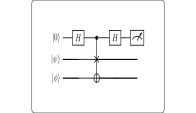
\includegraphics[width=0.6\textwidth]{../../images/quantum_kernel_circuit.svg}
\end{center}

\subsection{数学推导}

量子核函数：
\begin{equation}
K(x_i, x_j) = |\langle\phi(x_i)|\phi(x_j)\rangle|^2
\end{equation}

其中 $|\phi(x)\rangle$ 是量子特征映射。

\textbf{算法步骤}：
\begin{enumerate}
  \item 将数据编码到量子态 $|\phi(x)\rangle$
  \item 用 Swap 测试估计重叠度
  \item 计算核矩阵
\end{enumerate}

\subsection{几何解释}

量子核方法将数据映射到量子态空间，通过 Swap 测试计算核函数。

\section{代码详解}

\begin{lstlisting}[style=python]
from quonic.ml import quantum_kernel

# quantum_kernel(data, shots)
# data: input data points
# shots: number of measurements
result = quantum_kernel(data, shots=1024)

# result.kernel: kernel matrix
# result.fidelity: estimated fidelities
print(f"Kernel: {result.kernel}")
\end{lstlisting}

\section{进阶用法}

\subsection{场景 1：不同数据}

\begin{lstlisting}[style=python]
# Different datasets
data1 = [[0, 1], [1, 0], [1, 1]]
result1 = quantum_kernel(data1)

data2 = [[0, 0, 1], [1, 0, 0], [0, 1, 0]]
result2 = quantum_kernel(data2)
\end{lstlisting}

\section{适用场景}

\subsection{分类问题}

量子核方法可以用于分类问题，如量子 SVM。

\subsection{回归问题}

量子核方法可以用于回归问题，如量子高斯过程。

\section{常见问题}

\subsection{量子核方法的优势是什么？}

量子核方法可以在指数维的特征空间中计算核函数。

\subsection{量子核方法的局限性是什么？}

需要能够高效编码数据到量子态。

\section{学习路径}

\subsection{前置知识}
\begin{itemize}
  \item 核方法
  \item 量子态编码
  \item Swap 测试
\end{itemize}

\subsection{继续学习}
\begin{itemize}
  \item 量子 SVM
  \item 量子高斯过程
  \item 量子神经网络
\end{itemize}

\section{完整示例代码}

\subsection{示例 1：基本量子核方法}

\begin{lstlisting}[style=python]
from quonic.ml import quantum_kernel

data = [[0, 1], [1, 0]]
result = quantum_kernel(data)
print(f"Kernel: {result.kernel}")
\end{lstlisting}

\end{document}
